\documentclass{standalone}

% graphics
\usepackage{tikz}
\usepackage{pgfplots}
\usepackage{siunitx}

\begin{document}

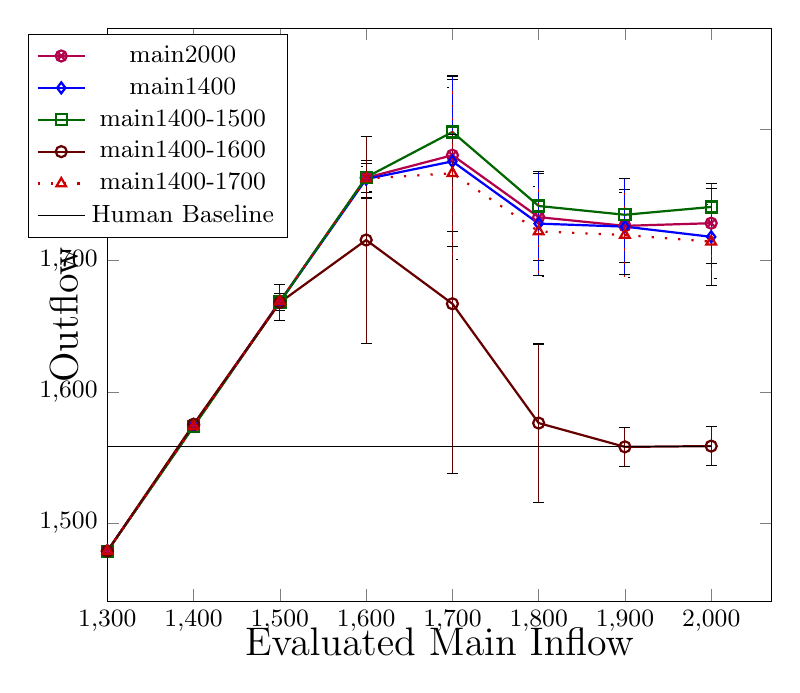
\begin{tikzpicture}[scale=1]
  \pgfplotsset{
      scale only axis,
      every x tick label/.append style={font=\small},
      every y tick label/.append style={font=\small},
	legend style={at={(-0.12,0.99)},anchor=north west}
  }

\begin{axis}[
    legend style={font=\small},
	ylabel={\Large Outflow},
	x label style={at={(axis description cs:0.5,-0.03)},anchor=north},
	y label style={at={(axis description cs:-0.030,0.5)}, anchor=south},
	xlabel={\Large Evaluated Main Inflow},
	xmin=1300
]

%densely dashed, 
%main2000_merge200
\addplot[mark=otimes, thick, mark options={solid, fill=red!60, mark size=2pt},
draw=red!70!blue, error bars/.cd, y dir=both, y explicit] table [x=a, y=b, y error=c] {
a	b   	c
1300 1478.74 1.70
1400 1574.35 2.44
1500 1668.85 2.71
1600 1762.88 11.06
1700 1780.06 57.92
1800 1732.93 33.10
1900 1726.31 27.80
2000 1728.32 30.39
};
\label{main2000}




% dashdotdotted,
%main1400-1400_merge200
\addplot[mark=diamond, thick, mark options={solid, fill=blue!40, mark size=2 pt}, draw=blue, error bars/.cd, y dir=both, y explicit] table [x=a, y=b, y error=c] {
a	b   	c
1300 1478.77 1.60
1400 1574.14 2.37
1500 1668.38 6.55
1600 1761.91 14.43
1700 1775.38 65.01
1800 1728.00 39.67
1900 1725.70 36.66
2000 1717.96 36.93
};
\label{main1400}

% error bars/.cd, y dir=both, y explicit,
%main1400-1500_merge200
\addplot[mark=square, thick, mark options={solid, fill=green!60, mark size=2 pt}, draw=black!60!green] table [x=a, y=b] {
a	b   	c
1300 1478.66 1.74
1400 1573.56 2.25
1500 1668.31 3.27
1600 1763.24 7.31
1700 1797.73 54.29
1800 1741.43 35.22
1900 1734.73 37.44
2000 1740.67 39.18
};
\label{main1400-1500}  

%densely dashed, 
%main1400-1600_merge200
\addplot[mark=o, thick, mark options={solid, fill=black!60!red, mark size=2pt}, draw=black!60!red, error bars/.cd, y dir=both, y explicit] table [x=a, y=b, y error=c] {
a	b   	c
1300 1478.77 1.68
1400 1575.36 2.33
1500 1667.95 13.85
1600 1715.54 78.51
1700 1667.02 128.87
1800 1576.19 60.22
1900 1558.08 14.70
2000 1558.66 14.96
};
\label{main1400-1600}

%densely dashed, 
%main1400-1700_merge200
\addplot[mark=triangle, thick, loosely dotted, mark options={solid, fill=red!60, mark size=2pt}, draw=black!20!red, error bars/.cd, y dir=both, y explicit] table [x=a, y=b, y error=c] {
a	b   	c
1300 1478.74 1.62
1400 1573.70 2.39
1500 1668.78 2.94
1600 1762.27 9.53
1700 1766.34 65.53
1800 1722.06 33.99
1900 1719.32 32.46
2000 1714.28 27.98
};
\label{main1400-1700}

%%densely dashed, 
%\addplot[mark=otimes, thick, mark options={solid, fill=red!60, mark size=2pt},
%draw=blue!10!green, error bars/.cd, y dir=both, y explicit] table [x=a, y=b, y error=c] {
%a	b   	c
%
%};
%\label{AVP90}
%
%
%%densely dashed, 
%\addplot[mark=otimes, thick, mark options={solid, fill=blue!60, mark size=2pt},
%draw=blue!10!red, error bars/.cd, y dir=both, y explicit] table [x=a, y=b, y error=c] {
%a	b   	c
%
%};
%\label{linearPPO}
%
\addplot[mark=none, black, samples=200] coordinates {(1300,1558.12)
(2000,1558.12)};
\label{Baseline}


\addlegendimage{/pgfplots/refstyle=main2000}
\addlegendentry{main2000}


\addlegendimage{/pgfplots/refstyle=main1400}
\addlegendentry{main1400}

\addlegendimage{/pgfplots/refstyle=main1400-1500}
\addlegendentry{main1400-1500}

\addlegendimage{/pgfplots/refstyle=main1400-1600}
\addlegendentry{main1400-1600}

\addlegendimage{/pgfplots/refstyle=main1400-1700}
\addlegendentry{main1400-1700}


%\addlegendimage{/pgfplots/refstyle=AVP90}
%\addlegendentry{AVP90}

%\addlegendimage{/pgfplots/refstyle=linearPPO}
%\addlegendentry{linearPPOAVP10}

\addlegendimage{/pgfplots/refstyle=Baseline}
\addlegendentry{Human Baseline}




\end{axis}
\end{tikzpicture}

\end{document}

